%!TEX root = ../rapport.tex

\begin{titlepage}
\newgeometry{top=2cm,bottom=2cm}

\newcommand{\HRule}{\rule{\linewidth}{0.5mm}} % Defines a new command for the horizontal lines, change thickness here

\center % Center everything on the page
 
%----------------------------------------------------------------------------------------
%   HEADING SECTIONS
%----------------------------------------------------------------------------------------


\includegraphics[scale=0.7]{Graphics/LOGO-IPSA.pdf}\\[2cm]

\Large Graduation Project \\[0.2cm] % Major heading such as course name
\large Autonomous Vehicles\\[2cm] % Minor heading such as course title

{\normalsize \today}\\[2cm]

%----------------------------------------------------------------------------------------
%   TITLE SECTION
%----------------------------------------------------------------------------------------

\HRule \\[0.5cm]
{ \Large \bfseries User Documentation}\\[0.2cm] % Title of your document
\HRule \\[2.5cm]


%----------------------------------------------------------------------------------------
%   LOGO SECTION
%----------------------------------------------------------------------------------------

 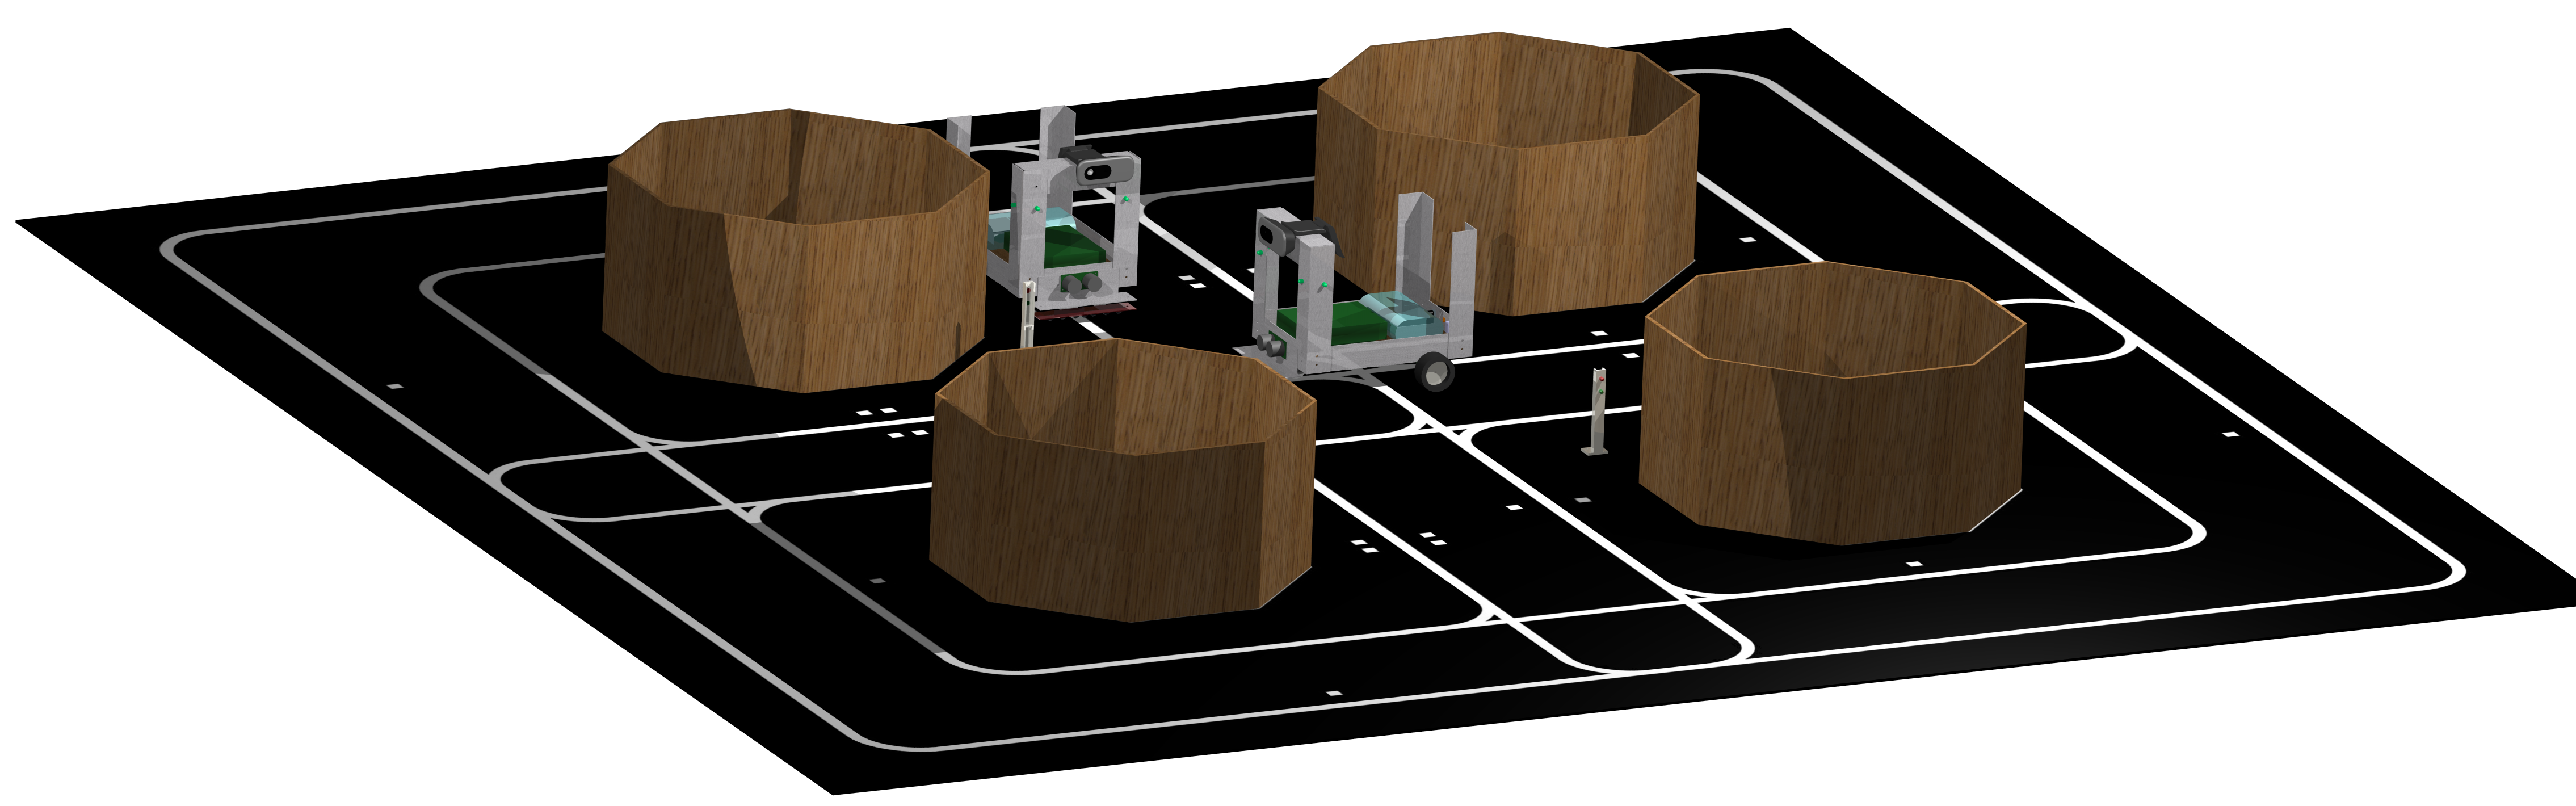
\includegraphics[scale=0.09]{Graphics/illu.png}\\[2.5cm]

%----------------------------------------------------------------------------------------
%   AUTHOR SECTION
%----------------------------------------------------------------------------------------
{\normalsize Auteurs:}\\
\small
BITON Guillaume \small(guillaume.biton@ipsa.fr)\\
MONNOT Maxime \small(maxime.monnot@ipsa.fr)\\
SON Kyeong Hwan \small(thsrudghks1@naver.com) [1cm]

 
%----------------------------------------------------------------------------------------

\vfill % Fill the rest of the page with whitespace

\restoregeometry

\end{titlepage}